\subsubsection{Tasks}

The following section has been enhanced with slides from Senior Principal Engineer Mattson Tim. He's a senior principal engineer at Intel, where he's been since 1993. His profile can be seen \href{https://www.intel.com/content/www/us/en/research/featured-researchers/tim-mattson.html}{here} and the slides are available online \href{https://www.openmp.org/wp-content/uploads/Intro_To_OpenMP_Mattson.pdf}{here}. He has also made an interesting \href{https://youtube.com/playlist?list=PLLX-Q6B8xqZ8n8bwjGdzBJ25X2utwnoEG&si=OBjyY4AI4zWfA-vB}{YouTube series} on the introduction to OpenMP.

\highspace
Tasks are \textbf{independent units of work}. They consist of: \emph{code to execute}, \emph{data environment}, and \emph{internal control variables} (ICV). \textbf{Threads perform the work of each task}. The runtime \textbf{system decides when to execute tasks}; each task can be deferred or executed immediately.

\highspace
In other words, an OpenMP \textbf{task is a block of code contained in a parallel region that can be executed simultaneously with other tasks in the same region}.

\highspace
Some useful terminology:
\begin{itemize}
    \item \textbf{\emph{Task construct}}. It identifies the \textbf{task directive plus the structured block}.
    
    \item \textbf{\emph{Task}}. It is the \textbf{package of code and instructions} for \textbf{allocating data} created when a \textbf{thread encounters a task construct}.
    
    \item \textbf{\emph{Task region}}. It is the dynamic sequence of \textbf{instructions generated by the execution of a task by a thread}.
\end{itemize}
Tasks are guaranteed to complete at thread barriers (using the \texttt{barrier} directive) or at task barriers (using the \texttt{taskwait} directive):
\begin{lstlisting}[language=C++, mathescape=true]
#pragma omp parallel // omp directive to parallel the code
{
    #pragma omp task // multiple $\textcolor{codegreen}{\emph{foo}}$ tasks created here, 
                     // one for each thread
    foo();
    #pragma omp barrier // all $\textcolor{codegreen}{\emph{foo}}$ tasks guaranteed 
                        // to be completed here
    #pragma omp single  // only one thread can access to 
                        // this piece of code
    {
        #pragma omp task // one $\textcolor{codegreen}{\emph{bar}}$ task created here
        bar();
    }
    // $\textcolor{codegreen}{\emph{foo}}$ task guaranteed to be completed here
}
\end{lstlisting}
\begin{examplebox}[: Fibonacci with tasks]
    Let us see a Fibonacci example of data scoping using the tasks. In the following code, we create the Fibonacci function and we create two tasks, but each task has a private variable and these variables are also used in the return statement:
    \begin{lstlisting}[language=C++]
int fib(int n) {
    int x, y;
    if(n < 2)
        return n;
    #pragma omp task
    x = fib(n-1);
    #pragma omp task
    y = fib(n-2);
    #pragma omp taskwait
    return x + y;
}\end{lstlisting}
    A good solution is to \dquotes{share} the \texttt{x} and \texttt{y} variables because we need both values to calculate the sum.
    \begin{lstlisting}[language=C++]
int fib(int n) {
    int x, y;
    if(n < 2)
        return n;
    #pragma omp task shared(x)
    x = fib(n-1);
    #pragma omp task shared(y)
    y = fib(n-2);
    #pragma omp taskwait
    return x + y;
}\end{lstlisting}
\end{examplebox}

\begin{flushleft}
    \textcolor{Green3}{\faIcon{check} \textbf{Main advantage}}
\end{flushleft}
Note the following code:
\begin{lstlisting}[language=C++]
// create a team of threads
#pragma omp parallel
{
    // one thread executes the single construct
    // and other threads wait at the implied 
    // barrier at the end of the single construct
    #pragma omp single
    { // block 1
        node *p = head;
        while(p) { // block 2
            // the single thread creates a task
            // with its own value for the pointer p
            #pragma omp task firstprivate(p)
                process(p);
            p = p -> next; // block 3
        }
        // execution moves beyond the barrier 
        // once all the tasks are complete
    }
}
\end{lstlisting}
The tasks have the \textbf{potential to parallelize irregular patterns and recursive function calls}. See Figure \ref{figure: openmp tasks 1} (page \pageref{figure: openmp tasks 1}) to understand how the runtime system can optimize execution using the tasks.
\begin{figure}[!htp]
    \centering
    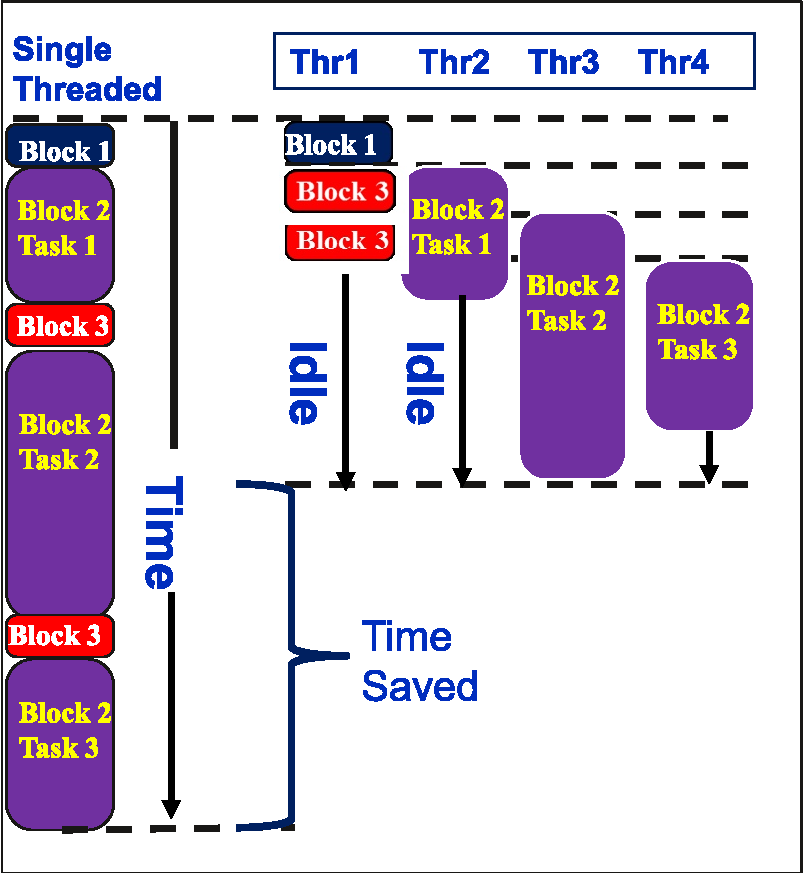
\includegraphics[width=.6\textwidth]{img/openmp-tasks-1.pdf}
    \caption{The main advantage of the tasks is to parallelize irregular patterns and recursive function calls.}
    \label{figure: openmp tasks 1}
\end{figure}

\newpage

\begin{flushleft}
    \textcolor{Green3}{\faIcon{bookmark} \textbf{Synchronization}}
\end{flushleft}
When a thread encounters a \texttt{task} construct, the task is created but not immediately executed. The tasks are guaranteed to be completed:
\begin{itemize}
    \item At a \textbf{barrier} (implicit or explicit)
    \item At \textbf{task synchronization points}:
    \begin{itemize}
        \item \texttt{taskwait} construct specifies a \textbf{wait on the completion of child tasks of the current task}.
        \marginpar{
            \href{https://www.openmp.org/spec-html/5.0/openmpsu94.html} {Doc. \faIcon{book}}
        }
        \begin{openmpbox}[: \texttt{pragma omp taskwait}]
        \begin{lstlisting}[language=C++]
#pragma omp taskwait\end{lstlisting}
        \end{openmpbox}

        \item \texttt{taskgroup} construct specifies a \textbf{wait on the completion of child tasks of the current task} (such as \texttt{taskwait}) and \textbf{their descendent tasks} (\underline{main difference}).
        \marginpar{
            \href{https://www.openmp.org/spec-html/5.0/openmpsu93.html\#x124-4690002.17.5} {Doc. \faIcon{book}}
        }
        \begin{openmpbox}[: \texttt{pragma omp taskgroup}]
        \begin{lstlisting}[language=C++]
#pragma omp taskgroup\end{lstlisting}
        \end{openmpbox}
    \end{itemize}
\end{itemize}
